\documentclass{standalone}
\usepackage{tikz}
\usepackage{pgfplots}
\usetikzlibrary{arrows.meta}

\begin{document}

\resizebox{8cm}{8cm}{%
    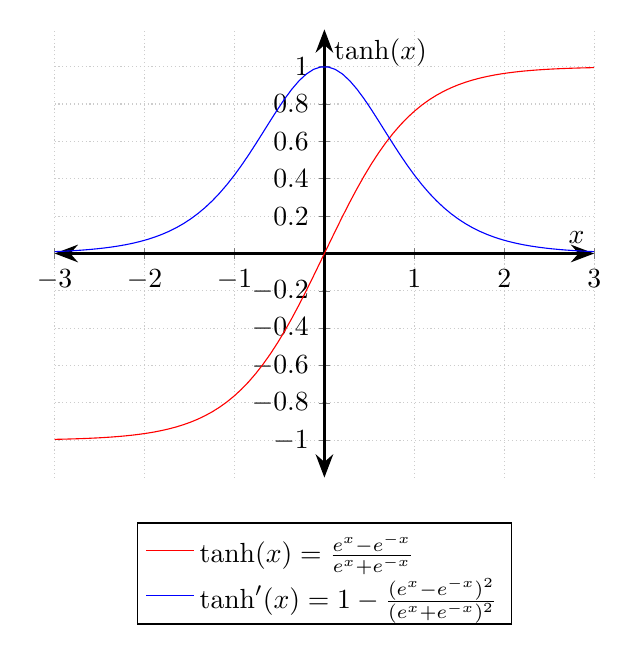
\begin{tikzpicture}
    \begin{axis}[
        title={},
        axis lines=middle,
        axis line style={Stealth-Stealth,very thick},
        xlabel=$x$,
        ylabel={$\tanh(x)$},
        xmin=-3,xmax=3,ymin=-1.2,ymax=1.2,
        xtick distance=1,
        ytick distance=1,
        grid=major,
        grid style={thin,densely dotted,black!20},
        % Numbers on axes
        xtick={-3,-2,-1,0,1,2,3},
        ytick={-1,-0.8,-0.6,-0.4,-0.2,0,.2,.4,.6,.8,1},
        % Legend
        legend style={
            at={(0.5,-0.1)}, % Position at the center bottom
            anchor=north, % Anchor the legend at the top
            cells={anchor=west} % Align the legend entries to the left
        }
    ]
    % Plot the sigmoid function
    \addplot[
        domain= -8:8,
        samples=200,
        color=red
        ]
        {(exp(x)-exp(-x))/(exp(x) + exp(-x))};

    % Plot the derivative of the sigmoid function
    \addplot[
        domain= -8:8,
        samples=200,
        color=blue
        ]
        {1-(exp(x)-exp(-x))^2/(exp(x) + exp(-x))^2};
    \addlegendentry{$\tanh(x) = \frac{e^x - e^{-x}}{e^x + e^{-x}}$}
    \addlegendentry{$\tanh'(x) = 1 - \frac{(e^x - e^{-x})^2}{(e^x + e^{-x})^2}$}
    \end{axis}
    \end{tikzpicture}
}

\end{document}